%██████╗ ███████╗██████╗      ██████╗██╗   ██╗██████╗ ██╗   ██╗███████╗███████╗
%██╔══██╗██╔════╝██╔══██╗    ██╔════╝██║   ██║██╔══██╗██║   ██║██╔════╝██╔════╝
%██████╔╝█████╗  ██████╔╝    ██║     ██║   ██║██████╔╝██║   ██║█████╗  ███████╗
%██╔══██╗██╔══╝  ██╔══██╗    ██║     ██║   ██║██╔══██╗╚██╗ ██╔╝██╔══╝  ╚════██║
%██████╔╝███████╗██║  ██║    ╚██████╗╚██████╔╝██║  ██║ ╚████╔╝ ███████╗███████║
%╚═════╝ ╚══════╝╚═╝  ╚═╝     ╚═════╝ ╚═════╝ ╚═╝  ╚═╝  ╚═══╝  ╚══════╝╚══════╝
%.:..:..:..:..:..:..:..:..:..:..:..:..:..:..:..:..:..:..:..:.
\section{BER Curves}
The standard \gls{OFDM} was simulated to obtain its \gls{BER} performance curves over the three channel models \emph{(Rayleigh, Rician and AWGN.)} These were compared to the variant's.

\begin{figure}[!h]
	\centerline{\resizebox{!}{0.9\textheight}{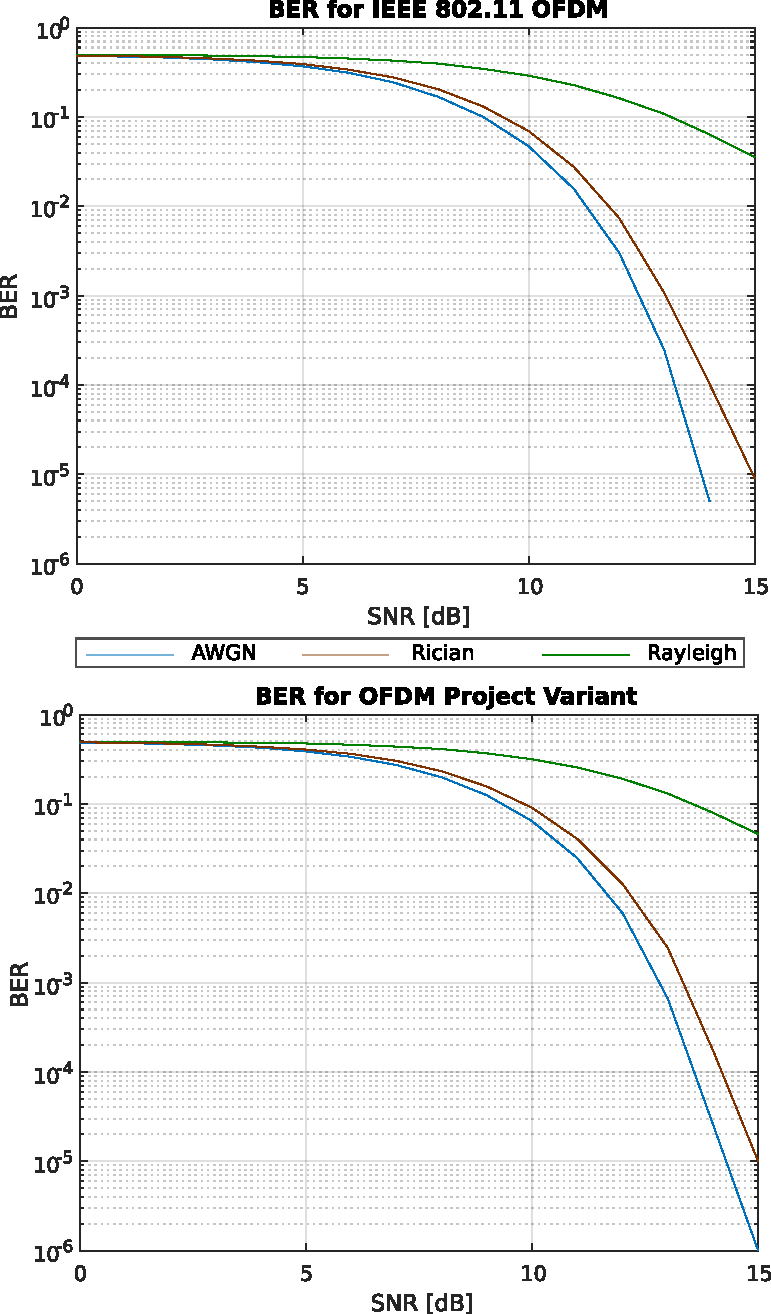
\includegraphics{Graphics/Results/stdandvariant.pdf}}}
	\caption{BER Performance Curves}
	\label{res:fig:berCurves}
\end{figure}

\pagebreak
